\section[Formal Analysis Using Alloy]{\hyperlink{toc}{Formal Analysis Using Alloy}}
	\label{sec:formalAnalysisUsingAlloy}
	The following section considers the essential properties and constraints identified for the specification of the problem and provides a formal model in which it is shown how they will be satisfied. The alloy modeling language is used to model the problem, and some possible worlds are also provided in order to clarify the most critical aspects. Before to read the alloy model, it is important to keep in mind that TPM actor is not considered in the worlds shown because they have only the functionality of visualizing and monitor farmers and agronomists. 
	
	\subsection[Alloy Model]{\hyperlink{toc}{Alloy Model}}
	\lstinputlisting[language=alloy]{Files/alloy/alloy.als}
	
	\FloatBarrier
	\newpage
	
	\subsection[First World]{\hyperlink{toc}{First World}}
	In this first world (\blueAutoref{fig:firstWorld}), the focus is on the registration, the types of users, how an account is managed. In the model illustrated each account has the same password, it is not restriction of the system but it is a possible scenario. Here the crucial aspect is: the farmers have only one location and every location belongs to a certain area, the agronomist has different daily plans for different dates where visits certain farmers, the agronomist is in charge of an area.
	
	\begin{figure}[h!]
		\centering
		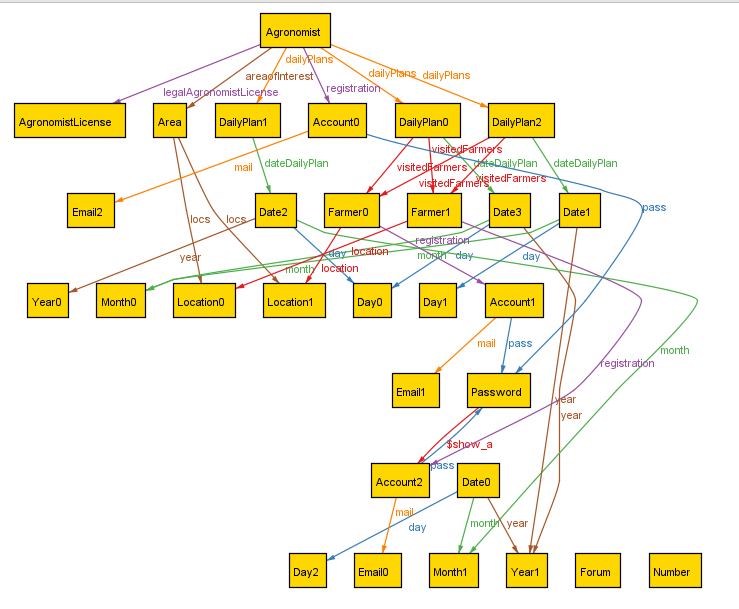
\includegraphics[scale=0.8]{Files/alloy/world1.png}
		\caption{\label{fig:firstWorld}First World generated}
	\end{figure}

	\FloatBarrier
	\newpage
	
	\subsection[Second World]{\hyperlink{toc}{Second World}}
	This second world (\blueAutoref{fig:secondWorld}) is similar to the previous one with additional aspects: the possibility for farmers to add production fields with their set of parameters and if it is harvested there exists the final date e the amount planted. For each production field we have updates, identified like feedbacks of the farmers
	
	\begin{figure}[hbtp]
		\centering
		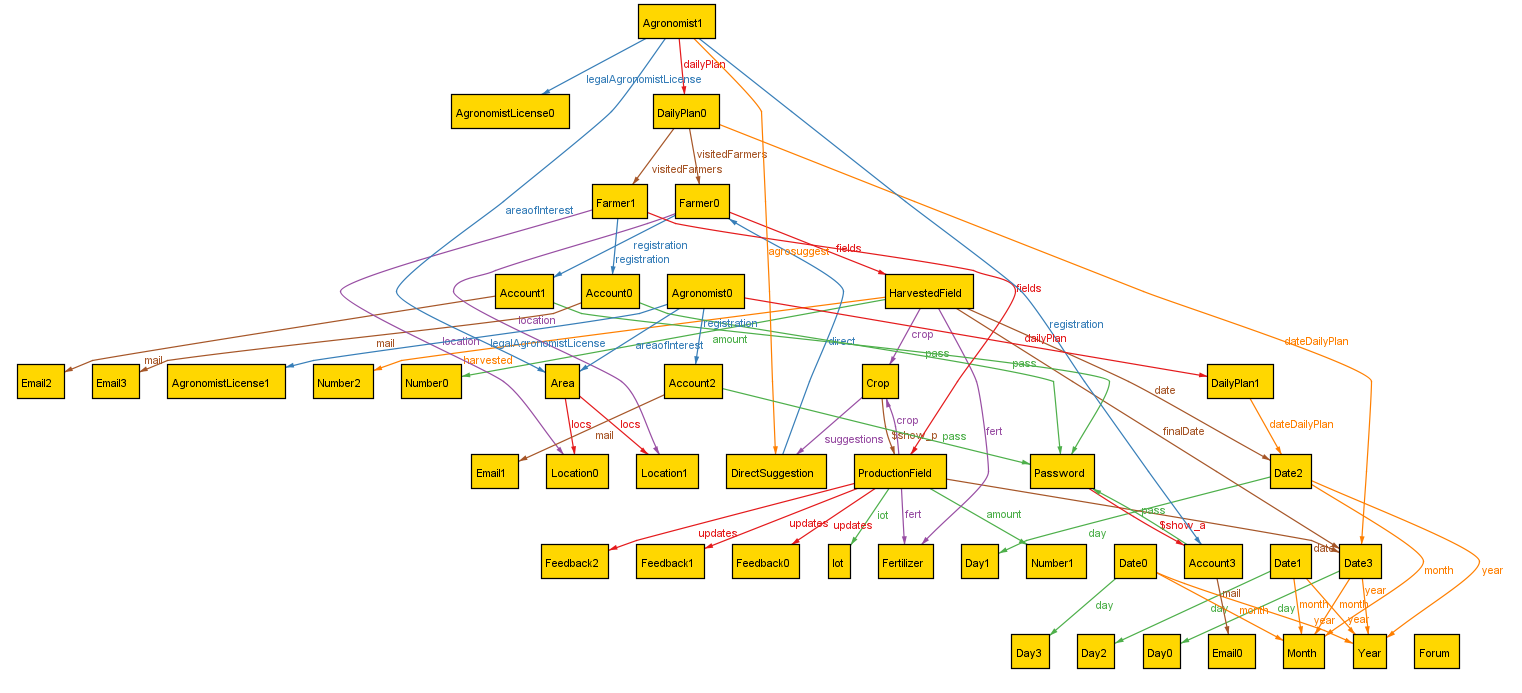
\includegraphics[scale=0.5, angle=90]{Files/alloy/world2.png}
		\caption{\label{fig:secondWorld}Second World Generated}
	\end{figure}
	
	\FloatBarrier
	\newpage
	\subsection[Third World]{\hyperlink{toc}{Third World}}
	The third example world (\blueAutoref{fig:thirdWorld}) focuses on the request function and on the forum interaction between farmers.
	
	\begin{figure}[h!]
		\centering
		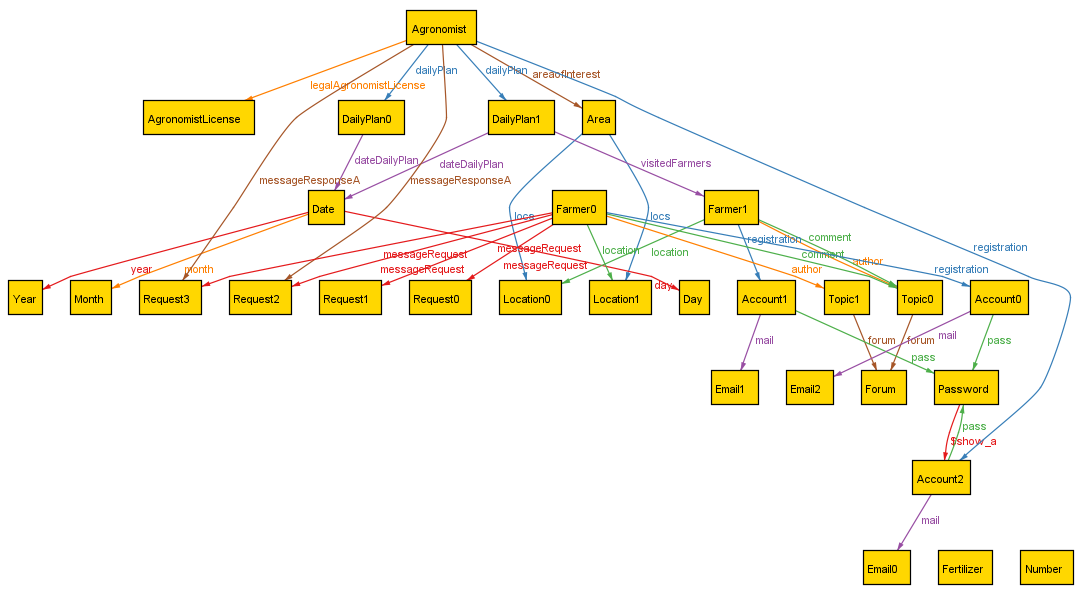
\includegraphics[scale=0.7, angle=90]{Files/alloy/world3.png}
		\caption{\label{fig:thirdWorld}Third World Generated}
	\end{figure}

	\FloatBarrier
	\newpage
	\subsection[Fourth]{\hyperlink{toc}{Fourth World}}
	The Fourth example world (\blueAutoref{fig:fourthWorld}) is also similar to the first world but it emphasizes the funcionality of the suggesstions. As described previously in the document we have two different types of suggestions: the farmer suggestion so written by a farmer and the direct suggestion written by an agronomist.
	
	\begin{figure}[h!]
		\centering
		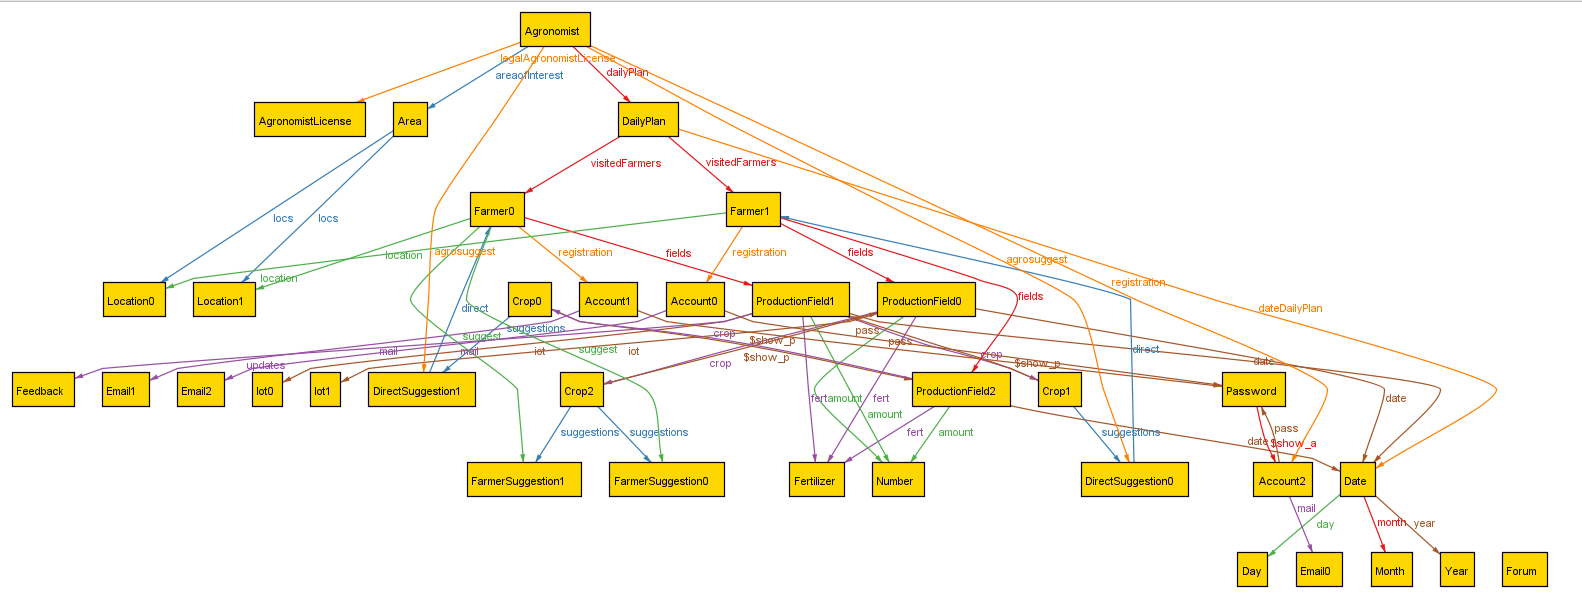
\includegraphics[scale=0.5, angle=90]{Files/alloy/world4.png}
		\caption{\label{fig:fourthWorld}Fourth World Generated}
	\end{figure}
	